\section{Three step protocol}
\begin{definition}[Three step protocol]
    Consider as follows:
    \begin{itemize}
        \item Let $k_{A}$ be the key of $A$, and $k_{B}$ be the key of $B$.
        \item Let $L_{A}$ be the lock of $A$, and $L_{B}$ be the lock of $B$.
        \item Assume that only the owner of the lock can open and close it.
        \item Assume that the two locks are independent and both unbreakable.
    \end{itemize}
    Then:
    \begin{itemize}
        \item[\textbf{Step 1 - User $A$:}] $A$ inserts the lock $L_{A}$ and sends the box to $B$. Now the box has only the key of $A$.
        \item[\textbf{Step 2 - User $B$:}] $B$ inserts the lock $L_{B}$ and sends the box to $B$. Now the box has both the locks.
        \item[\textbf{Step 3 - User $A$:}] $A$ removes the lock $L_{A}$ and sends the box to $B$. Now the box has only the key of $B$. $B$ can now receive securely the box that contains the secret, because he's the only one that can open the lock $L_{B}$.
    \end{itemize}
\end{definition}
This protocol can easily implemented by using the XOR operator as the enciphering function, as it satisfies the assumptions of this protocol.
\begin{figure}[h]
    \centering
    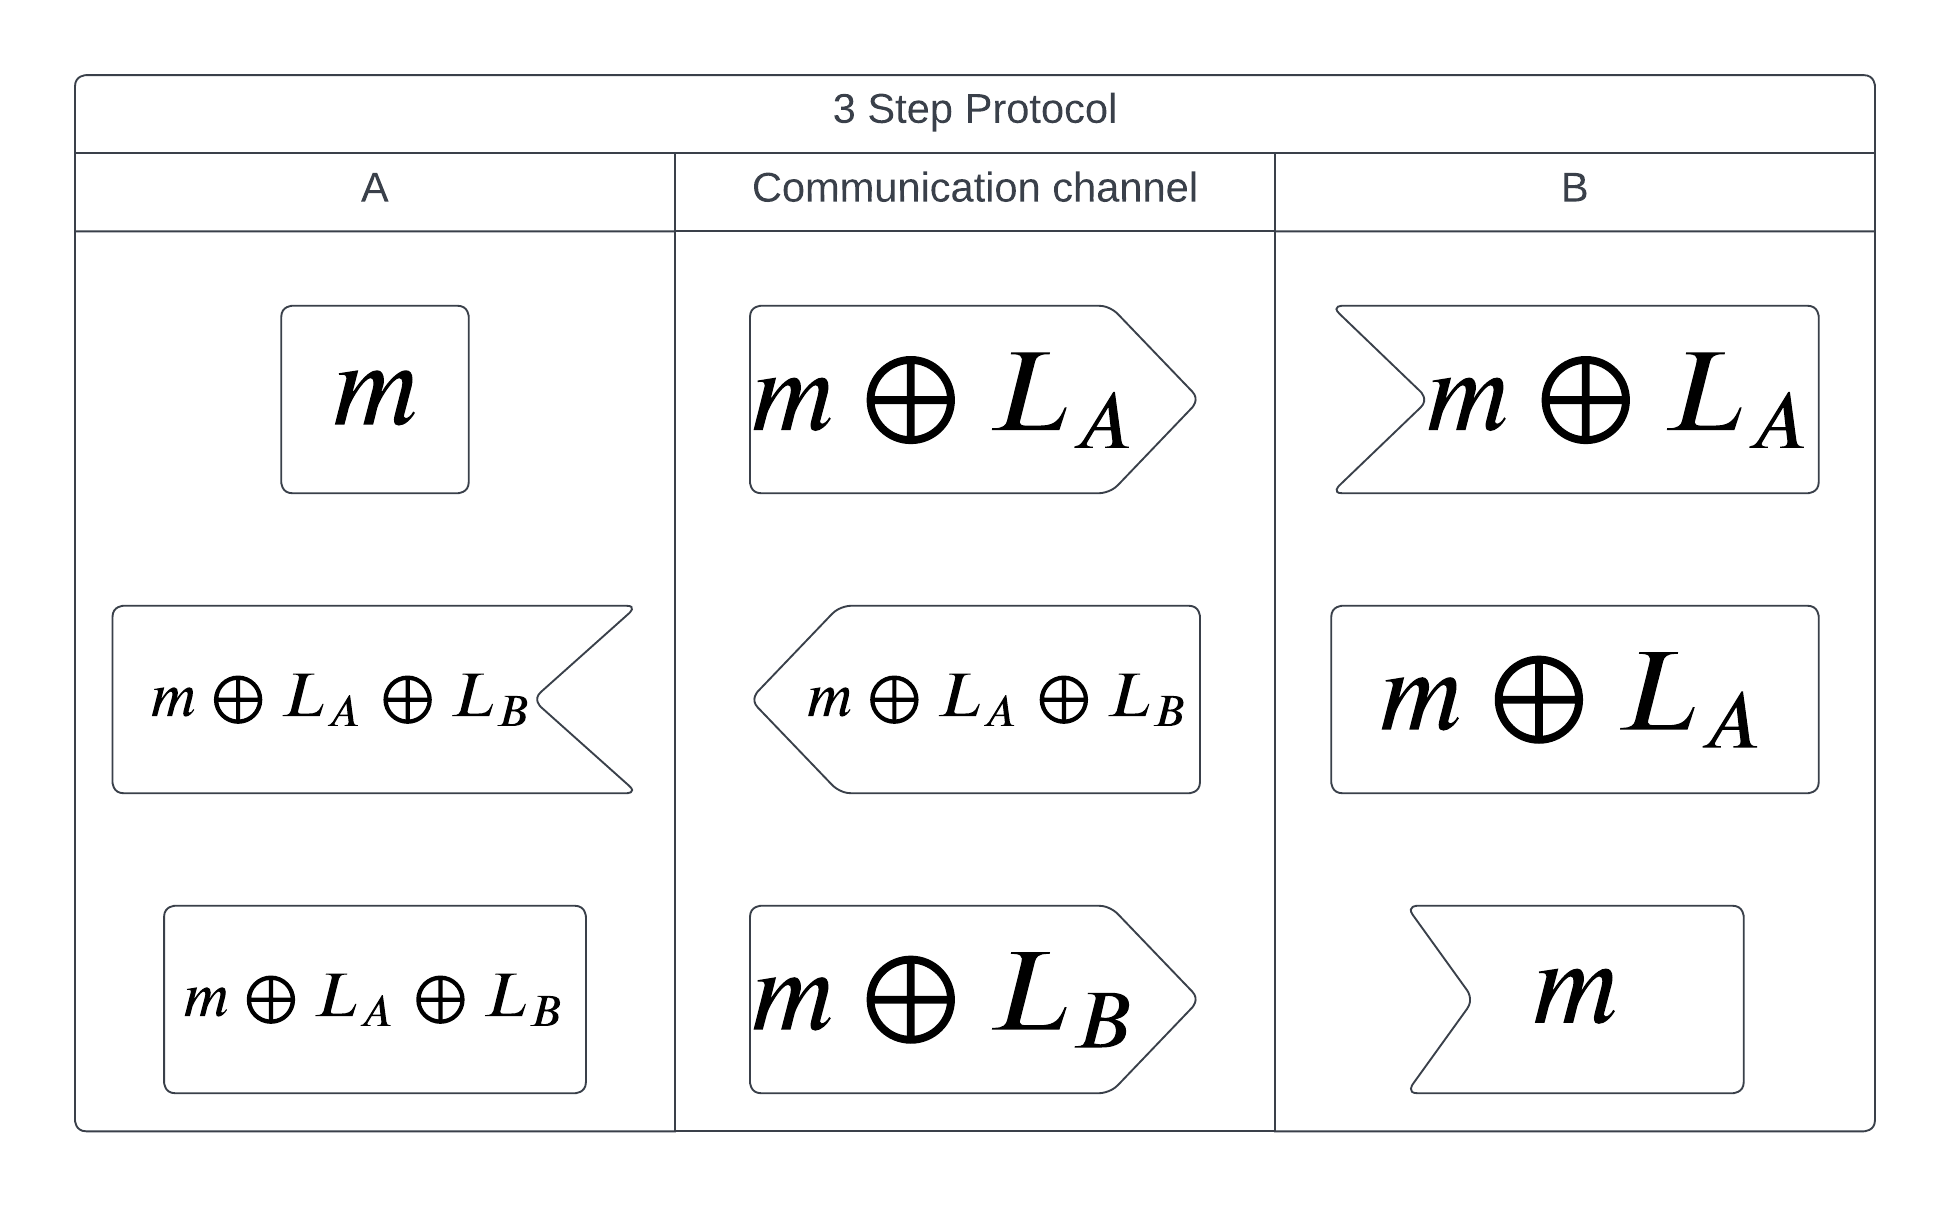
\includegraphics[width=\textwidth]{img/KeyExc_3SP.png}
    \caption{Key Exchange with the Three-Steps-Protocol.}
\end{figure}

\section{Diffie-Helman algorithm}
This method allows to exchange the keys for the communication over an unsecure channel. This methods assumes that computing the discrete logarithm is hard.\newline
Let $p$ be a large prime number, and $g$ the generator of $\mathbb{Z}_{p}^{*} = <g>$. $p, g$ are public available.
Let $A, B$ be the users of the communication. Then:
\begin{itemize}
    \item $A$ generates randomly $a \in \mathbb{Z}_{p-1}$ and sends $g^{a} \bmod p \in \mathbb{Z}_{p}^{*}$.
    \item $B$ generates randomly $b \in \mathbb{Z}_{p-1}$ and sends $g^{b} \bmod p \in \mathbb{Z}_{p}^{*}$.
    \item $A$ computes $(g^{b})^{a}$ and $B$ computes $(g^{a})^{b}$. This now allows them to compute respectively $b, a$ by using the logarithm.
    \item Since $a, b$ are secret, the keys are exchanged successfully.
\end{itemize}

The intruder can only have access to $p, g$ (that are public) and $g^{a}, g^{b}$. Computing $g^{ab}$ is called the Diffie-Helman problem.\newline
If the intruder can solve this problem, that translates to the Discrete Logarithm Problem\ref{discrete_logarithm_prob}, then he has access to $a, b$.

\begin{figure}[h]
    \centering
    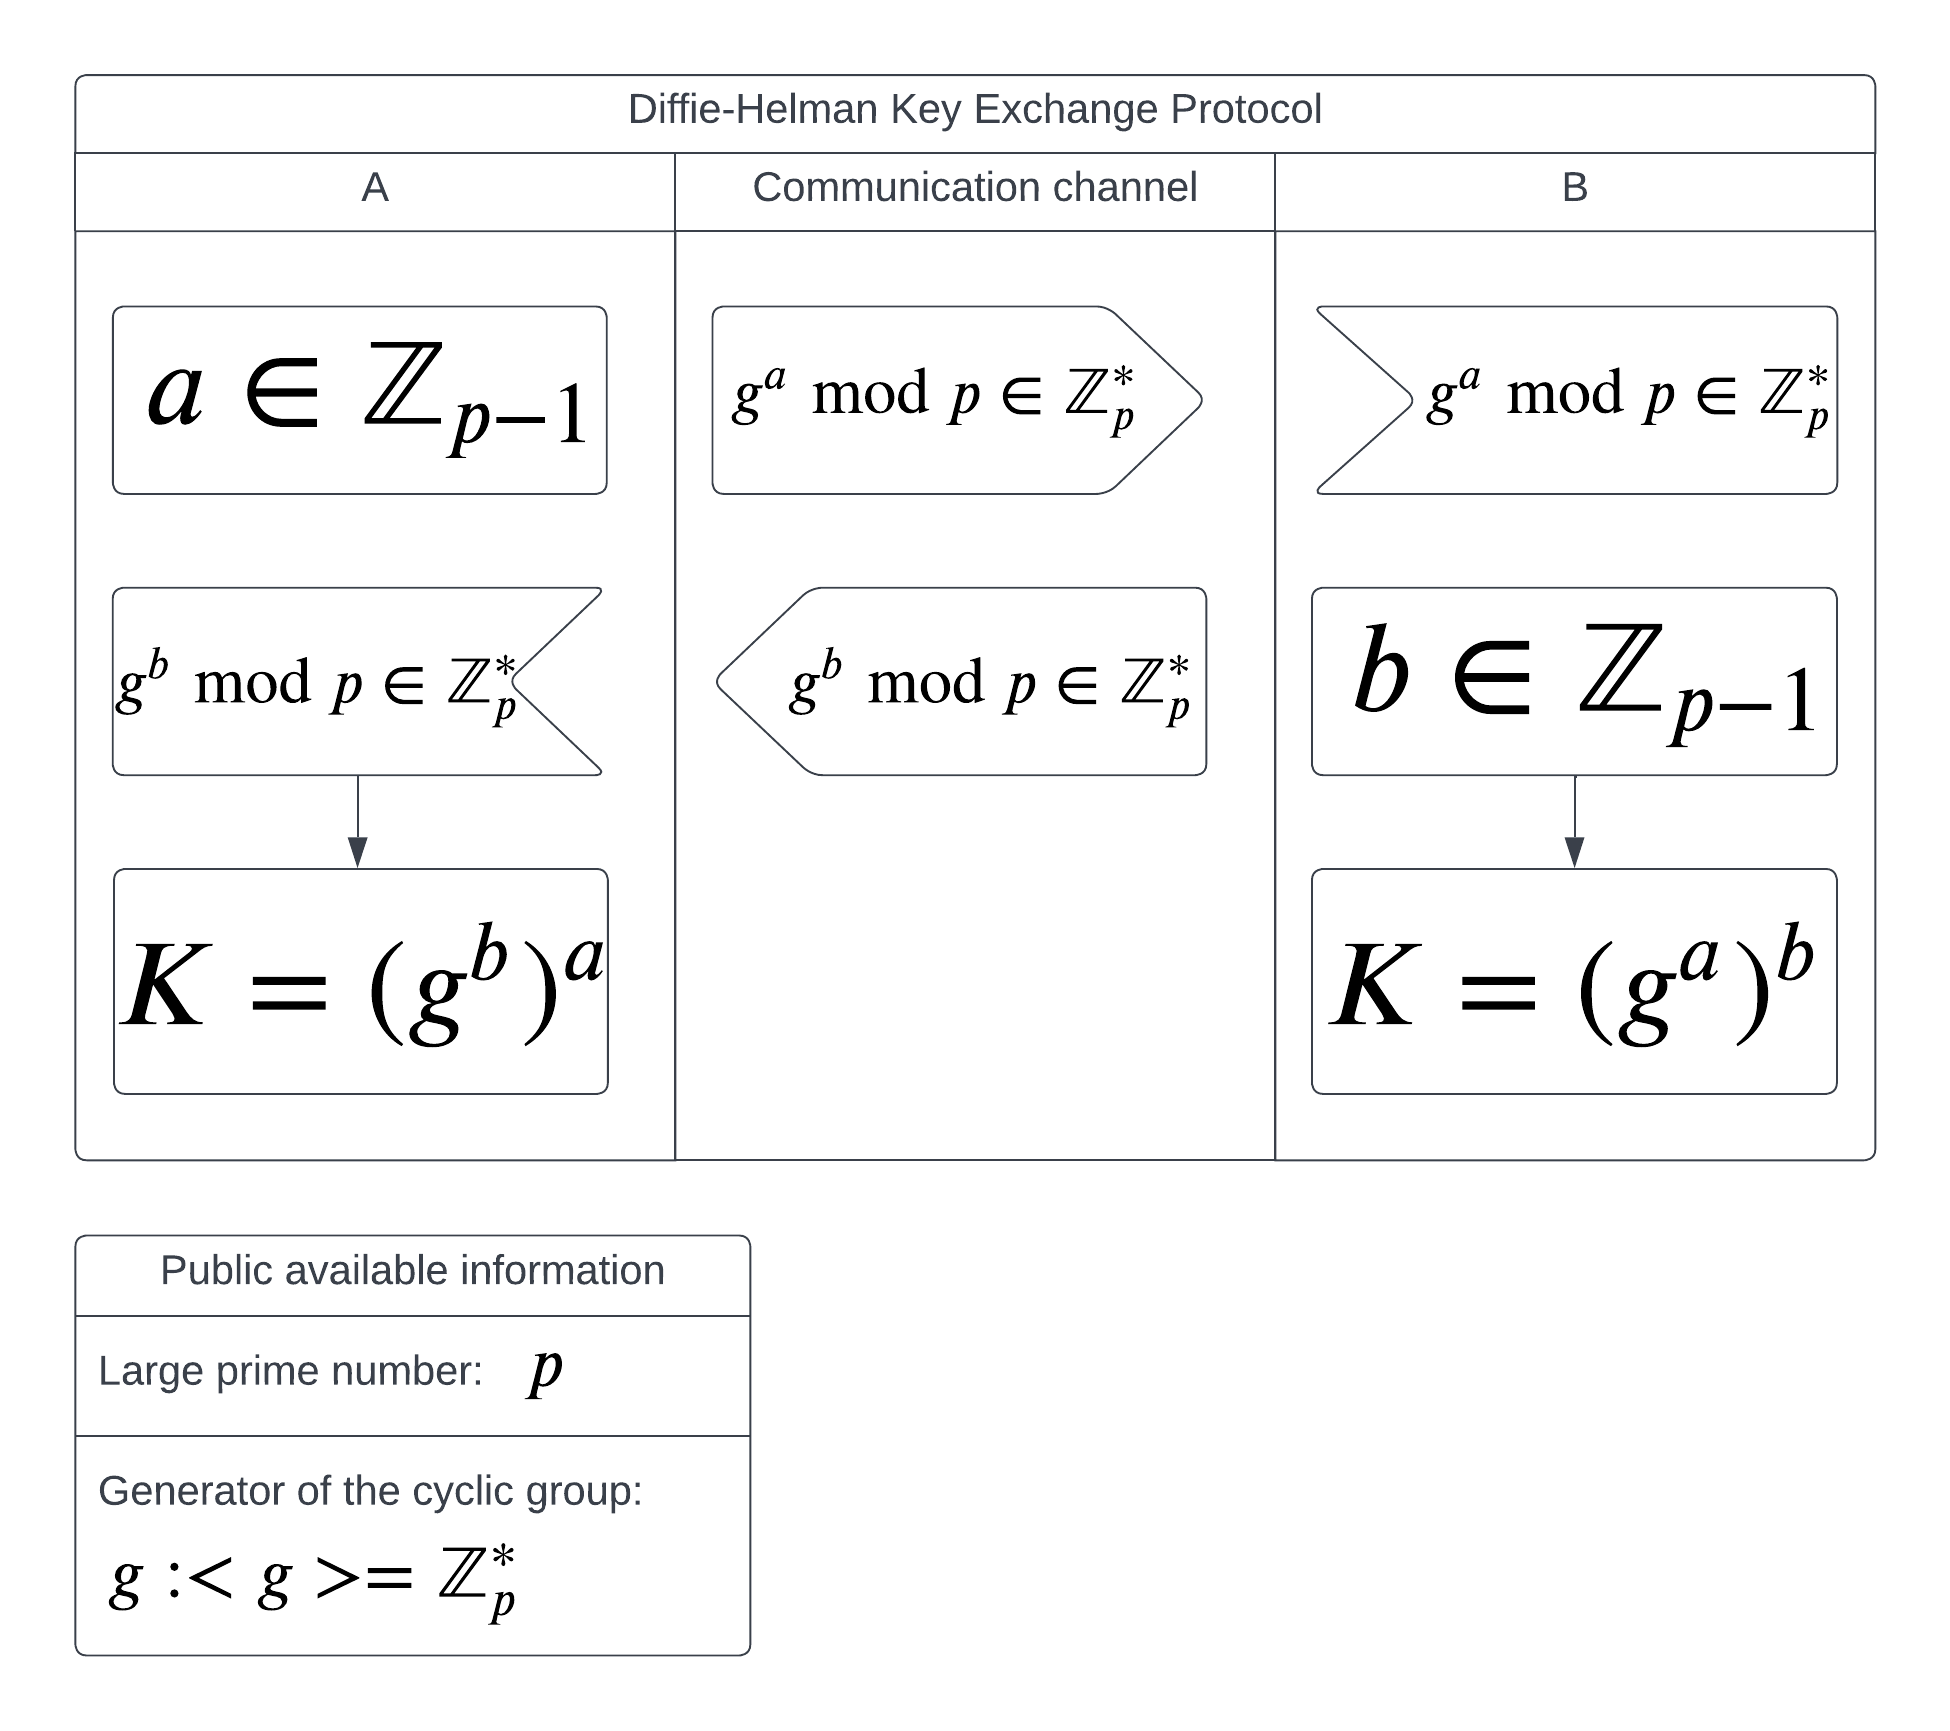
\includegraphics[width=\textwidth]{img/KeyExc_DHP.png}
    \caption{Key Exchange with the Three-Steps-Protocol.}
\end{figure}
